\documentclass[journal]{vgtc}                % final (journal style)
%\documentclass[review,journal]{vgtc}         % review (journal style)
%\documentclass[widereview]{vgtc}             % wide-spaced review
%\documentclass[preprint,journal]{vgtc}       % preprint (journal style)

%% Uncomment one of the lines above depending on where your paper is
%% in the conference process. ``review'' and ``widereview'' are for review
%% submission, ``preprint'' is for pre-publication, and the final version
%% doesn't use a specific qualifier.

%% Please use one of the ``review'' options in combination with the
%% assigned online id (see below) ONLY if your paper uses a double blind
%% review process. Some conferences, like IEEE Vis and InfoVis, have NOT
%% in the past.

%% Please use the ``preprint''  option when producing a preprint version
%% for sharing your article on an open access repository

%% Please note that the use of figures other than the optional teaser is not permitted on the first page
%% of the journal version.  Figures should begin on the second page and be
%% in CMYK or Grey scale format, otherwise, colour shifting may occur
%% during the printing process.  Papers submitted with figures other than the optional teaser on the
%% first page will be refused. Also, the teaser figure should only have the
%% width of the abstract as the template enforces it.

%% These few lines make a distinction between latex and pdflatex calls and they
%% bring in essential packages for graphics and font handling.
%% Note that due to the \DeclareGraphicsExtensions{} call it is no longer necessary
%% to provide the the path and extension of a graphics file:
%% 
\includegraphics{diamondrule} is completely sufficient.
%%
\ifpdf%                                % if we use pdflatex
  \pdfoutput=1\relax                   % create PDFs from pdfLaTeX
  \pdfcompresslevel=9                  % PDF Compression
  \pdfoptionpdfminorversion=7          % create PDF 1.7
  \ExecuteOptions{pdftex}
  \usepackage{graphicx}                % allow us to embed graphics files
  \DeclareGraphicsExtensions{.pdf,.png,.jpg,.jpeg} % for pdflatex we expect .pdf, .png, or .jpg files
\else%                                 % else we use pure latex
  \ExecuteOptions{dvips}
  \usepackage{graphicx}                % allow us to embed graphics files
  \DeclareGraphicsExtensions{.eps}     % for pure latex we expect eps files
\fi%

%% it is recomended to use ``\autoref{sec:bla}'' instead of ``Fig.~\ref{sec:bla}''
\graphicspath{{figures/}{pictures/}{images/}{./}} % where to search for the images

\usepackage{microtype}                 % use micro-typography (slightly more compact, better to read)
\PassOptionsToPackage{warn}{textcomp}  % to address font issues with \textrightarrow
\usepackage{textcomp}                  % use better special symbols
\usepackage{mathptmx}                  % use matching math font
\usepackage{times}                     % we use Times as the main font
\renewcommand*\ttdefault{txtt}         % a nicer typewriter font
\usepackage{cite}                      % needed to automatically sort the references
%% We encourage the use of mathptmx for consistent usage of times font
%% throughout the proceedings. However, if you encounter conflicts
%% with other math-related packages, you may want to disable it.
\usepackage{amsmath,amsfonts,amssymb,pxfonts,eulervm,xspace}
\usepackage{mathrsfs} % math script fonts
\usepackage{tabulary}
\usepackage{subfig} %ieee does not like subfigure
\usepackage{multicol}
\usepackage{tikz}
\usetikzlibrary{cd} % commutative diagrams
\usepackage[switch]{lineno}
\usepackage{minted}
\setminted[python]{fontsize=\scriptsize, 
                   linenos,
                   numbersep=8pt,
                   autogobble, 
                   frame=lines,
                   framesep=3mm} 
\usepackage{notation} % move this later


%% In preprint mode you may define your own headline. If not, the default IEEE copyright message will appear in preprint mode.
%\preprinttext{To appear in IEEE Transactions on Visualization and Computer Graphics.}

%% In preprint mode, this adds a link to the version of the paper on IEEEXplore
%% Uncomment this line when you produce a preprint version of the article 
%% after the article receives a DOI for the paper from IEEE
%\ieeedoi{xx.xxxx/TVCG.201x.xxxxxxx}

%% If you are submitting a paper to a conference for review with a double
%% blind reviewing process, please replace the value ``0'' below with your
%% OnlineID. Otherwise, you may safely leave it at ``0''.
\onlineid{0}

%% declare the category of your paper, only shown in review mode
\vgtccategory{Research}
%% please declare the paper type of your paper to help reviewers, only shown in review mode
%% choices:
%% * algorithm/technique
%% * application/design study
%% * evaluation
%% * system
%% * theory/model
\vgtcpapertype{Theory/Model}

%% Paper title.
\title{Topological Equivariant Artist Model}

%% This is how authors are specified in the journal style

%% indicate IEEE Member or Student Member in form indicated below
\author{Hannah Aizenman, Thomas Caswell, Michael Grossberg}
\authorfooter{
%% insert punctuation at end of each item
\item
 Hannah Aizenman and Michael Grossberg are with the Computer Science department, City College of New York. E-mail: haizenman@ccny.cuny.edu, mgrossberg@ccny.cuny.edu.
\item
 Thomas Caswell is with National Synchrotron Light Source II, Brookhaven National Lab E-mail: tcaswell@bnl.gov.
}

%other entries to be set up for journal
\shortauthortitle{ \MakeLowercase{\textit{et al.}}: Topological Equivariant Artist Model}
%\shortauthortitle{Firstauthor \MakeLowercase{\textit{et al.}}: Paper Title}

%% Abstract section.
\abstract{ A critical aspect of data visualization is that the graphical representation of data is expected to match the structure of the data; this fails, for example, when order is not preserved in representations of ordinal data or proportional distance for numerical data or when discrete data is plotted on a line plot or interpolated as an image. In this work, we propose the topological equivariant artist model (TEAM), wherein we formalize the expectations of attributes and continuity matching using the mathematical notion of equivariance and by modeling data and graphics as fiber bundles. Specifically, our model introduces measurement scale preserving maps on the fiber that transform data components (variables) into visual channels and a continuity preserving map on the base space that transforms dataset connectivity into graphical elements. Furthermore, TEAM has a sum operator to allow for building composite visualizations. We illustrate the application of the model through case studies of a scatter plot, line plot, and heatmap and show that this model can be implemented with a small prototype.} 

% end of abstract

%% Keywords that describe your work. Will show as 'Index Terms' in journal
%% please capitalize first letter and insert punctuation after last keyword
% http://ieeevis.org/year/2021/info/call-participation/paper-keywords
\keywords{Taxonomy, Models, Frameworks, Theory }

%% ACM Computing Classification System (CCS). 
%% See <http://www.acm.org/class/1998/> for details.
%% The ``\CCScat'' command takes four arguments.
%https://www.acm.org/publications/computing-classification-system/1998/top
\CCScatlist{ % not used in journal version
 \CCScat{I.3.6}{Computer Graphics}%
{Methodology and Techniques}{Graphics data structures and data types};}

%% A teaser figure can be included as follows
\teaser{
  \centering
  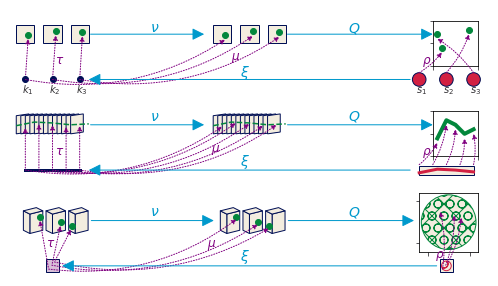
\includegraphics[width=\linewidth]{teaser.png}
  \caption{Visualizations consist of topologically equivariant maps. There is a set of monoid action equivariant maps from data components to visual components \vchannel\ that are then reduced via \vmark\ into a single graphic, and there is a deformation retraction \vindex\ from graphic continuity to data continuity.}
  \label{fig:teaser}
}

%% Uncomment below to disable the manuscript note
%\renewcommand{\manuscriptnotetxt}{}

%% Copyright space is enabled by default as required by guidelines.
%% It is disabled by the 'review' option or via the following command:
% \nocopyrightspace


\vgtcinsertpkg

%%%%%%%%%%%%%%%%%%%%%%%%%%%%%%%%%%%%%%%%%%%%%%%%%%%%%%%%%%%%%%%%
%%%%%%%%%%%%%%%%%%%%%% START OF THE PAPER %%%%%%%%%%%%%%%%%%%%%%
%%%%%%%%%%%%%%%%%%%%%%%%%%%%%%%%%%%%%%%%%%%%%%%%%%%%%%%%%%%%%%%%%

\begin{document}
\linenumbers %linenumbers for comments [make sure to remove later]
%% The ``\maketitle'' command must be the first command after the
%% ``\begin{document}'' command. It prepares and prints the title block.

%% the only exception to this rule is the \firstsection command
\firstsection{Introduction}
\maketitle
The aim of this work is to rearchitecture Matplotlib to take advantage of developments in software design, data structures, and visualization to improve consistency, reusability, and discoverability, so domain specific tool developers can build structure preserving visualization tools. The contribution of this work is 
\begin{enumerate}
  \item topology preserving relationship between data and graphic via continuous maps
  \item property preservation from data component to visual representation as equivariant maps that carry a homomorphism of monoid actions
  \item functional oriented visualization tool architecture built on the mathematical model to demonstrate the utility of the model
  \item prototype of the architecture built on Matplotlib's infrastructure to demonstrate the feasibility of the model.
\end{enumerate}

\section{Related Work}
The underlying structure and semantics of visualization are by definition reflected in visual representations \cite{friendlyBriefHistoryData2008}, whether through direct mappings from data into visual elements or via figurative representations that have meaning due to their similarity to external concepts \cite{byrneAcquiredCodesMeaning2016}. The components of a visual representation were first codified by Bertin\cite{bertinSemiologyGraphicsDiagrams2011a}, and the notion that the properties of the data and visual representation match is the basis of most evaluations of visualization. Expressiveness, as defined by Mackinlay \cite{mackinlayAUTOMATICDESIGNGRAPHICAL1987, mackinlayAutomatingDesignGraphical1986} is a measure of how much of the structure any map can encode. A fully expressive component is one that is equivariant since it has preserved all the structure in the data. 
Models of visualization evaluate this equivariance and how elements built in the model can be composed to build more complex visualizations. Mackinlay's \textit{A Presentation Tool} (APT) introduced the notion of visualizations having syntax and semantics \cite{mackinlayAutomatingDesignGraphical1986} and Wilkenson described the grammar of this language \cite{wilkinsonGrammarGraphics2005}. This grammar oriented approach allows users to describe how to compose visual elements into a graphical design \cite{wongsuphasawatNavigatingWideWorld2021}, while we are proposing a framework for building those elements. This same limitation is explicitly stated in the functional dependency model of visualization developed by Sugibuchi\cite{sugibuchiFramwork2009} and evident in Vickers' category theory oriented framework in which semiotics are commutative. The algebraic process model by Kindlmann and Scheideggar proposes that the data and visualization transformations are commutative; while similar to our framework, it is missing any explicit mention of continuity. 

On the other hand, most information visualization tools are explicitly tuned to specific continuity \cite{HeerSoftware2006,toryRethinkingVisualizationHighlevel2004}. For example, the relational database is core to tools influenced by APT, such as
Tableau\cite{StoltePolaris2002,hanrahanVizQL2006,MackinlayShowme2007} and the Grammar of Graphics\cite{wilkinsonGrammarGraphics2005} inspired ggplot\cite{wickhamGgplot2ElegantGraphics2016a}, Vega\cite{satyanarayanDeclarativeInteractionDesign2014} and Altair\cite{vanderplasAltairInteractiveStatistical2018}. Images underpin scientific visualization tools such as Napari\cite{nicholas_sofroniew_2021_4533308} and ImageJ\cite{schneiderNIHImageImageJ2012} and the digital humanities oriented ImagePlot\cite{studiesCulturevisImageplot2021} macro; the need to visualize and manipulate graphs has spawned tools like Gephi\cite{bastianGephiOpenSource2009}, Graphviz\cite{ellsonGraphvizOpenSource2002}, and Networkx\cite{HagbergExploringNetwork2008}. Neither the table nor image nor graph model on its own supports all the data types a typical general purpose visualization library needs to support; instead libraries such as Matplotlib\cite{hunterMatplotlib2DGraphics2007} and Vtk\cite{hanwellVisualizationToolkitVTK2015, geveci2012vtk} and D3 \cite{bostockDataDrivenDocuments2011} explicitly carry around different data representations for all the different types of visualizations they support.  Where libraries with a single core data structure have very consistent APIs, VTK, D3 and Matplotlib APIs can be rather inconsistent as every visualization has a different notion of how the data is structured.

Fiber bundles are a generalized abstraction proposed by Butler to encode the continuity of the data separately from the variable information \cite{butlerVisualizationModelBased1989,butlerVectorBundleClassesForm1992}. Since Butler's model lacks a robust way of describing variables, we fold in Spivak's Simplicial formulation of databases \cite{spivakDatabasesAreCategories2010,spivakSIMPLICIALDATABASES} to incorporate a schema like description of the variables. One way of describing the binding between the schame and the continuinity is using the notion of structural \textit{keys} with associated \textit{values} proposed by Munzner\cite{munznerVisualizationAnalysisDesign2014}. Unlike Munzner's model where the semantic meaning of the key is tightly coupled to the index of the value, our model considers keys to be a reference to topology. This allows the metadata to be altered, for example by changing the coordinate system or time resolution, without imposing new semantics on the underlying structure. 


\section{Topological Equivariant Artist Model}
\label{sec:math}
We introduce the notion of an artist $\mathscr{\vartist}$ as an equivariant map from data to graphic
\begin{equation}
    \label{eq:artist}
    \mathscr{\vartist}: \mathscr{\dtotal} \rightarrow \mathscr{\gtotal}
\end{equation}
that carries a homomorphism of monoid actions $\varphi: \monoid \rightarrow \monoid^{\prime}$ \cite{cegarraCohomologyMonoidsOperators2019}, which are discussed in detail in \autoref{sec:math:data:monoid}. Given \monoid\ on data $\mathscr{\dtotal}$ and $\monoid^{\prime}$ on graphic $\mathscr{\gtotal}$, we propose that artists $\mathscr{\vartist}$ are equivariant maps 
\begin{equation}
\mathscr{\vartist}(m\cdot \delement) = \varphi(m)\cdot\mathscr{\vartist}(\delement) 
\end{equation}
such that applying a monoid action $m \in \monoid$ to the data $\delement \in \mathscr{\dtotal}$ input to $\mathscr{\vartist}$ is equivalent to applying a monoid action $\varphi(\monoid) \in \monoid^{\prime}$ to the graphic $\vartist(\delement) \in \mathscr{\gtotal}$ output of the artist.
We model the data $\mathscr{\dtotal}$, graphic $\mathscr{\gtotal}$, and intermediate visual encoding $\mathscr{\vtotal}$ stages of visualization as topological structures that encapsulate types of variables and continuity; by doing so we can develop implementations that keep track of both in ways that let us distribute computation while still allowing assembly and dynamic update of the graphic. 
\subsection{Data Bundle}
\label{sec:math:data}
Building on Butler's proposal of using fiber bundles as a common data representation structure for visualization data\cite{butlerVectorBundleClassesForm1992, butlerVisualizationModelBased1989}, a fiber bundle is a tuple $(\dtotal,\,\dbase,\,\pi ,\,\dfiber)$ defined by the projection map $\pi$
\begin{equation}
    \label{eq:fiber_bundle}
    \begin{tikzcd}
        \dfiber \arrow[r, hook] & \dtotal \arrow[r, "\pi"] & \dbase
    \end{tikzcd}
\end{equation}
that binds the components of the data in \dfiber\ to the continuity represented in \dbase. By definition fiber bundles are locally trivial\cite{spanier1989algebraic,LocallyTrivialFibre}, meaning that over a localized neighborhood we can dispense with extra structure on \dtotal\ and focus on the components and continuity.

\subsubsection{Fiber Space: Variables}
\label{sec:math:data:fiber}
\begin{figure}[htb]
  \centering % avoid the use of \begin{center}...\end{center} and use \centering instead (more compact)
  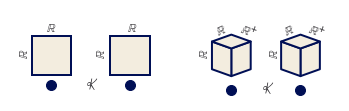
\includegraphics[width=\columnwidth]{fiber.png}
  \caption{These two datasets have the same base space \dbase\ of discrete points, but the square is a visual representation of the fiber space  $\dfiber=\reals\times\reals$, while the cube is a representation of $\dfiber=\reals\times\realsp\times\reals$}
  \label{fig:math:data:fiber}
\end{figure}

To formalize the structure of the data components, we use notation introduced by Spivak \cite{spivakSIMPLICIALDATABASES} that binds the components of the fiber to variable names. Spivak constructs a set \ftotal\ that is the disjoint union of all possible objects of types $\{\ftype_0, \ldots, \ftype_m\} \in \ftypes$, where \ftypes\ are the data types of the variables in the dataset. He then defines the single variable set \fttype\ 
\begin{equation}
    \label{eq:data_types}
    \begin{tikzcd}
        \fttype \arrow[r] \arrow[d, "\pi_{\fsection}"'] & \ftotal \arrow[d, "\pi"] \\
        \fnames \arrow[r, "\fsection"']                          & \ftypes       
    \end{tikzcd}
\end{equation}
which is \ftotal\ restricted to objects of type \ftype\ bound to variable name \fname. The \fttype\ lookup is by name to specify that every component is distinct, since multiple components can have the same type \ftype. Given \fsection, the fiber for a one variable dataset is
\begin{equation}
    \dfiber = \ftotal_{\fsection(\fname)} = \ftotal_{\ftype} 
\end{equation}
where \fsection\ is the schema binding variable name \fname\ to its datatype \ftype. A dataset with multiple variables has a fiber that is the cartesian cross product of $\ftotal_{\fsection}$ applied to all the columns:
\begin{equation}
F = \ftotal_{\fsection(\fname_{1})}\times \ldots \ftotal_{\fsection(\fname_{i})} \ldots\times \ftotal_{\fsection(\fname_{n})}
\end{equation}
which is equivalent to 
\begin{equation}
    \label{eq:math:data:fiber:decompose}
    \dfiber= \dfiber_{0} \times \ldots \times \dfiber_{i}\times\ldots\times \dfiber_{n}
\end{equation}
which allows us to decouple \dfiber\ into components $\dfiber_i$. Each component of \dfiber\ is a dimension of the topological fiber space, as illustrated in \autoref{fig:math:data:fiber}. The space $\dfiber=\reals\times\reals$ encodes that the dataset has two quantative continuous variables, while $\dfiber=\reals\times\reals\realsp$ encodes a dataset with three quantative contunous variables, one of which must be positive. 

\subsubsection{Equivariant Variable Properties: Monoid Actions}
\label{sec:math:data:monoid}
While structure on a set of values is often described algebraically as operations or through the actions of a group, for example Steven's measurement scales \cite{stevensTheoryScalesMeasurement1946, leaFormalizationMeasurementScale}, we generalize to monoids to support partial orderings. A partial ordering allows for multiple measurement values to have the same rank\cite{fongInvitationAppliedCategory2019}, which is useful for visualizing many types of multi indicator systems\cite{bruggemannRankingPrioritizationMultiindicator2011}. 

A monoid \cite{Monoid2021} $\monoid$ is a set with an associative binary operator $\ast:\monoid \times \monoid\rightarrow \monoid$. A monoid has an identity element $e\in \monoid$ such that $e\ast a= a \ast e = a$ for all $a \in \monoid$. As defined on a component of \dfiber, a left monoid action \cite{SemigroupAction2021,nlab:action} of $\monoid_i$ is a set $\dfiber_i$ with an action $\bullet: \monoid\times \dfiber_i \rightarrow \dfiber_i$ with the properties:
\begin{align*}
    \textbf{associativity}\;& \text{for all } f,g \in \monoid_i \text{ and } x\in \dfiber_i,\, f\bullet(g\bullet x) = (f\ast g) \bullet x\\
    \textbf{identity}\;& \text{for all } x\in \dfiber_i, e\in \monoid_i,\,  e\bullet x = x 
\end{align*}
As with the fiber \dfiber\, the total monoid space \monoid\ is the cartesian product
\begin{equation}
\monoid= \monoid_{0} \times \ldots \times \monoid_{i}\times \ldots \times\ldots \monoid_{n}
\end{equation}
of each monoid $\monoid_{i}$ on $\dfiber_{i}$.  The monoid is also added to the specification of the fiber $(\fname_i,\, \ftype_i,\, \fttype\, \monoid_i)$

Defining the monoid actions on the components serves as the basis for identifying the invariance\cite{kindlmannAlgebraicProcessVisualization2014} that must be preserved in the visual representation of the component. A secondary advantage of defining structure in terms of monoids is that they are commonly found in functional programming because they specify compositions of transformations \cite{yorgeyMonoidsThemeVariations, stievenMonadJustMonoid2020}.

\subsubsection{Base Space: Continuity}
\label{sec:math:data:base}
 The base space \dbase\ is way to express how the records in \dtotal\ are connected to each other, for example if they are discrete points or if they lie in a 2D continous surface. Formally \dbase\ is the quotient space of \dtotal\, meaning it is the finest space\cite{aurouxMath131Introduction} such that every $\dbasepoint \in \dbase$ has a corresponding fiber $\dfiber_k$\cite{QuotientSpaceTopology2020}. Our model formulates \dbase\ as akin to an indexing space into \dtotal\ that describes the structure of \dtotal.  
 
 \begin{figure}[htb]
  \centering % avoid the use of \begin{center}...\end{center} and use \centering instead (more compact)
  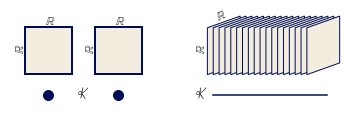
\includegraphics[width=\columnwidth]{base.png}
  \caption{These two datasets have the same fiber space  $\dfiber=\reals\times\reals$, but the left dataset has a discrete continuity while the right is 1D continuous over the interval $\left[0,1\right]$.}
  \label{fig:math:data:base}
 \end{figure}

 As illustrated in ~\autoref{fig:math:data:base}, \dbase\ can have any number of dimensions, can be continuous or discrete, and is somewhat independent of the dimensions of the fiber. As with fibers and monoids, we can decompose the total space into components $\pi:\dtotal_i\rightarrow \dbase$ where
 \begin{equation}
    \label{eq:math:data:base:decompose}
     \pi:\dtotal_1\oplus\ldots\oplus \dtotal_i \oplus\ldots \oplus \dtotal_n \rightarrow \dbase
 \end{equation}
 which is a decomposition of \dfiber. The \dbase\ remains the same because the connectivity of records does not change just because there are fewer elements in each record. By encoding this continuity in the model as \dbase\, the data model now explicitly carries information about its structure such that the implicit assumptions of the visualization algorithms are now explicit. The explicit topology is a concise way of distinguishing visualizations that appear identical, for example heatmaps and images.  

 \subsubsection{Section: Values}
 \label{sec:math:data:section}
 \begin{figure}[htb]
  \centering % avoid the use of \begin{center}...\end{center} and use \centering instead (more compact)
  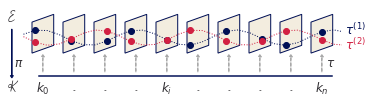
\includegraphics[width=\columnwidth]{fiberbundle.png}
  \caption{Each section in the fiber bundle is a unique continuous map from base space to fiber encoding the set of records in the dataset. The two sections, $\dsection^{(1)}$ and $\dsection^{(2)}$, shown here are in the set of global sections $\Gamma(\dtotal)$.}
  \label{fig:math:data:section}
 \end{figure}

 While the projection function $\pi:\dtotal \rightarrow\dbase$ ties together the base space \dbase\ with the fiber \dfiber, a section $\dsection: \dbase\rightarrow \dtotal$ encodes a dataset. A section function takes as input location $\dbasepoint \in \dbase$ and returns a record $\delement \in \dtotal$. For any fiber bundle, there exists a map
 \begin{equation}
     \begin{tikzcd}
         \dfiber \arrow[r, hook] & \dtotal \arrow[d, "\pi"'] \\
                           & \dbase \arrow[u, "\dsection"', bend right]
     \end{tikzcd}
 \end{equation}
  such that $\pi(\dsection(\dbasepoint)) = \dbasepoint$. The set of all global sections is denoted as $\Gamma(\dtotal)$. As illustrated in \autoref{fig:math:data:section}, the section is a continuous mapping from a location $\dbasepoint \in \dbase$ on the base space to a record $\delement \in \dfiber$ in the fiber. Assuming a trivial fiber bundle $\dtotal = \dbase \times \dfiber$, the section is 
 \begin{equation}
     \label{eq:section_return}
     \dsection(\dbasepoint) = (\dbasepoint, (g_{\dfiber_{0}}(\dbasepoint), \ldots, g_{\dfiber_{n}}(\dbasepoint)))
 \end{equation}
 where $g: \dbase \rightarrow \dfiber$ is the index function into the fiber component. This formulation of the section also holds on locally trivial sections of a non-trivial fiber bundle. As with \autoref{eq:math:data:fiber:decompose} and \autoref{eq:math:data:base:decompose}, \dsection\ can be decomposed into components 
 \begin{equation}
 \label{eq:math:data:section:decompose}
 \dsection= (\dsection_0,\ldots, \dsection_i, \dots, \dsection_n) 
 \end{equation}
 where each section $\dsection_i$ maps into a record on a component $\dfiber_i \in \dfiber$. This allows for accessing the data component wise in addition to accessing the data in terms of its location over \dbase.

 \subsubsection{Sheafs: Gluing Sections }
 \label{sec:math:data:sheaf}
 The restriction maps of a sheaf describe how local sections $\iota^{*}\dsection$ over a neighborhood $U$ around \dbasepoint\ can be glued into larger sections \cite{ghristElementaryAppliedTopology2014,ghristHomologicalAlgebraData2018}. This puts a continuous structure on local sections, which allows for defining a section over a subset in \dbase. The inclusion map $\iota: U \rightarrow \dbase$ pulls \dtotal\ over $U$ 
 \begin{equation}
     \label{eq:sheaf}
     \begin{tikzcd}
         \iota^*\dtotal \arrow[d, "\pi"'] \arrow[r, "\iota^*", hook]             & \dtotal \arrow[d, "\pi"']                  \\
         U \arrow[r, "\iota", hook] \arrow[u, "\iota^{*}\dsection"', bend right] & \dbase \arrow[u, "\dsection"', bend right]
     \end{tikzcd}
 \end{equation}
 such that the pulled back $\iota^*\dsection$ only contains records over $U \subset \dbase$. Gluing together $\iota^*\dsection$ sections is necessary for navigation techniques such as pan and zoom\cite{NekrasovskiEvaluationPanZoom2006} and dynamically updated visualizations such as sliding windows\cite{crouchDynamicGraphsSlidingwindow2013,chuTimeSeriesSegmentation1995}. 

 \subsection{Graphic Bundle}
 \label{sec:math:graphic}  
We introduce a graphic bundle to hold the essential information necessary to render a graphical design constructed by the artist. As with the data, we can represent the target graphic as a section \gsection\ of a bundle  $(\gtotal, \gbase, \pi, \gfiber)$
\begin{equation}
  \begin{tikzcd}[ampersand replacement=\&]
      \gfiber \arrow[r, hook] \& \gtotal \arrow[d, "\pi"'] \\
                        \& \gbase \arrow[u, "\gsection"', bend right]
  \end{tikzcd}
\end{equation}
where \gsection\ is the fully encoded graphic. To fully specify the visual characteristics of the image, we construct a fiber \gfiber\ that is an infinite resolution version of the target space. Typically \gtotal\ is trivial and therefore sections can be thought of as mappings into \gfiber. In this work, we assume a 2D opaque image $\gfiber=\reals^5$ with elements $(x,\, y,\, r,\, g,\, b) \in \gfiber$ such that a rendered graphic only consists of 2D position and color. By abstracting the target display space as \gfiber, the model can support different targets, such as a 2D screen or 3D printer. 

\subsubsection{Equivariant Topology: Graphic Base Space}
\label{sec:math:graphic:base}
\begin{figure}[htb]
  \centering % avoid the use of \begin{center}...\end{center} and use \centering instead (more compact)
  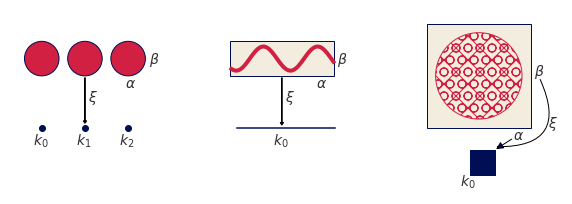
\includegraphics[width=\columnwidth]{retraction_maps.png}
  \caption{The 0D scatter \dbasepoint\ and 1D line \dbasepoint\ are thickened into \gbase\ with coordinates $\gbasepoint=(\gx, \gy)$ that are a region in an idealized 2D screen. The image has the same dimension in \gbase\ as in \dbase.}
  \label{fig:math:graphic:base}
 \end{figure}

Just as the \dbase\ encodes the connectivity of the records in the data, we propose an equivalent \gbase\ that encodes the connectivity of the rendered elements of the graphic. Formally, we require that \dbase\ be a deformation retract\cite{RetractionTopology2020} of \gbase\ so that \dbase\ and \gbase\ have the same homotopy. The surjective map $\vindex: \gbase \rightarrow \dbase$ 
\begin{equation}
    \begin{tikzcd}
        \dtotal \arrow[d, "\pi"'] & \gtotal \arrow[d, "\pi"'] \\
        \dbase                   & \gbase \arrow[l, "\vindex"']
    \end{tikzcd}
\end{equation}
goes from region $\gbasepoint \in \gbase_{\dbasepoint}$ to its associated point $\gbasepoint$. While \gbase\ must have the same continuity as \dbase\, it is sometimes the  thickened version shown in \autoref{fig:math:graphic:base}. This thickening is necessary when the dimensionality of \dbase\ is less than the dimensionality of the target display. For example, a \dbasepoint\ that is 0D in \dbase\ cannot be represented on screen unless it is thickened to 2D to encode the connectivity of the points in \gfiber\ that visually represent the record at \dbasepoint. 

\subsection{Artist}
The topological artist \vartist\ is a monoid equivariant sheaf map from the sheaf on a data bundle \dtotal\ which is $\mathcal{O}(\dtotal)$ to the sheaf on the graphic bundle \gtotal, $\mathcal{O}(\gtotal)$. 
\begin{equation}
    \vartist: \mathcal{O}(\dtotal) \rightarrow \mathcal{O}(\gtotal)
\end{equation}
While \vartist\ can usually construct graphical elements solely with the data in \dsection, some visualizations, such as line, may also need some finite number $n$ of derivatives, which is captured by the jet bundle $\mathcal{J}^n$ \cite{JetBundle2020,musilovaCalculusVariationsJet2016} with $\mathcal{J}^{0}(\dtotal)=\dtotal$. In this work, we at most need $\mathcal{J}^{2}(\dtotal)$ which is the value at \dsection\ and its first and second derivatives; therefore the artist takes as input the jet bundle $\dtotal^{\prime}=\mathcal{J}^{2}(\dtotal)$. 

Specifically, \vartist\ is the equivariant map from $\dtotal^{\prime}$ to a specific graphic $\gsection \in \Gamma(H)$ 
\begin{equation}
    \label{eq:math:artist:diagram}
    \begin{tikzcd}
        \dtotal^{\prime} \arrow[r, "\vchannel"] \arrow[rd, "\pi"'] & \vtotal \arrow[d, "\pi"] & \vindex^*\vtotal \arrow[r, "\vmark"] \arrow[d, "\vindex^*\pi"'] \arrow[l, "\vindex^*"'] & \gtotal \arrow[ld, "\pi"] \\
                                              & \dbase                  & \gbase \arrow[l, "\vindex"']                                              &                    
        \end{tikzcd}
\end{equation}
where the input can be point wise $\dsection(\dbasepoint)\mid \dbasepoint \in \dbase$. The visual bundle $(\vtotal,\,\dbase,\,\pi ,\,\vfiber)$ is the latent space of possible parameters of a visualization type, such as a scatter or line plot. As with the data and graphic bundles, the visual bundle is  defined by the projection map $\pi$
\begin{equation}
    \begin{tikzcd}[ampersand replacement=\&]
        \vfiber \arrow[r, hook] \& \vtotal \arrow[d, "\pi"'] \\
                          \& \dbase \arrow[u, "\vsection"', bend right]
    \end{tikzcd}
\end{equation}
where \vsection\ is the visual variable encoding\cite{bertinSemiologyGraphicsDiagrams2011a} of the data section \dsection. The visual fiber \vfiber\ is defined in terms of the input parameters of the visualization library's plotting functions; by making these parameters explicit components of the fiber, we can build consistent definitions and expectations of how these parameters behave. 

In \autoref{eq:math:artist:diagram}, the encoders $\vchannel:\dtotal^{\prime} \rightarrow \vtotal$ convert the data components to visual components. The continuity map $\vindex:\gbase \rightarrow \dbase$ then pulls back the visual bundle \vtotal\ over \gbase. Then the assembly function $\vmark: \vtotalpull \rightarrow \gtotal$ composites the fiber components of \vtotalpull\ into a graphic in \gtotal. This functional decomposition of the visualization artist facilitates building reusable components at each stage of the transformation because the equivariance constraints are defined on \vchannel, \vmark, and \vindex. We name this map the artist as that is the analogous part of the  Matplotlib\cite{hunterArchitectureOpenSource} architecture that builds visual elements.

\subsubsection{Visual Component Maps}
\label{sec:math:artist:nu}
\begin{figure}[htb]
  \centering
  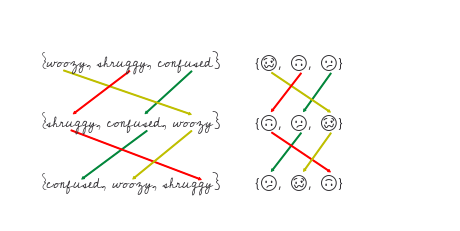
\includegraphics[width=\columnwidth]{equivariance_nu.png}
  \caption{In this artist, \vchannel\ maps the strings to the emojis. This \vchannel\ is equivariant because the monoid actions, represented by the colored arrows, are the same on the input \dsection\ and output \vsection\ sets.}
  \label{fig:math:artist:nu}
\end{figure}
 We define the visual transformers \vchannel\ 
\begin{equation}
  \label{eq:math:artist:nu}
  \{\vchannel_{0}, \ldots, \vchannel_{n}\}: \{\dsection_{0}, \ldots, \dsection_{n}\} \mapsto \{\vsection_{0}, \ldots, \vsection_{n}\}
\end{equation}
as the set of equivariant maps $\vchannel_i: \dsection_i \mapsto \vsection_i$. Given $\monoid_i$ is the monoid action on $\dtotal_i$ and that there is a monoid ${\monoid_i}^{\prime}$ on $\vtotal_i$, then there is a monoid homomorphism from $\varphi:\monoid_i \rightarrow {\monoid_i}^{\prime}$ that \vchannel\ must preserve. As mentioned in \autoref{sec:math:data:monoid}, monoid actions define the structure on the fiber components and are therefore the basis for equivariance. 
A validly constructed \vchannel\ is one where the diagram of the monoid transform $m$ commutes such that 
\begin{equation}
  \label{eq:math:artist:nu_commute}
\begin{tikzcd}
  \dtotal_i \arrow[r] \arrow[r, "\vchannel_i"] \arrow[d, "m_{\delement}"'] & \vtotal_i \arrow[d, "m_{\velement}"] \\
  \dtotal_i \arrow[r, "\vchannel_i"]                           & \vtotal_i               
\end{tikzcd}
\end{equation}
In general, the data fiber $\dfiber_{i}$ cannot be assumed to be of the same type as the visual fiber $\vfiber_{i}$ and the actions of \monoid\ on $\dfiber_{i}$ cannot be assumed to be the same as the actions of $\monoid^{\prime}$ on \vfiber; therefore an equivariant $\vchannel_i$ must satisfy the constraint  
\begin{equation}
\vchannel_i(m_{\delement}(\dtotal_i)) = \varphi(m_{\delement})(\vchannel_i(\dtotal_i))
\end{equation} 
such that $\varphi$ maps a monoid action on data to a monoid action on visual elements. However, we can construct a monoid action of \monoid\ on $\vfiber_{i}$ that is compatible with a monoid action of \monoid\ on $\dfiber_{i}$. We can compose the monoid actions on the visual fiber $\monoid^{\prime} \times \vfiber_{i} \rightarrow \vfiber_{i}$ with the homomorphism $\varphi$ that takes \monoid\ to $\monoid^{\prime}$. This allows us to define a monoid action on \vfiber\ of \monoid\ that is $(m, \velement) \rightarrow \varphi(m)\bullet\velement$. Therefore, without a loss of generality, we can assume that an action of \monoid\ acts on $\dfiber_{i}$ and on $\vfiber_{i}$ compatibly such that $\varphi$ is the identity function. 

The \vchannel\ illustrated in \autoref{fig:math:artist:nu} is an equivariant mapping from \textbf{Strings} to emojis, as seen in the identical actions, represented as arrows, on the data and emojis. More generally, for the Steven's scales\cite{stevensTheoryScalesMeasurement1946} an equivariant \vchannel\ has the following properties
\begin{table}[H]
  \begin{tabulary}{\columnwidth}{llL}
      nominal & permutation &  $\text{if } \delement_1 \neq \delement_2 \text{ then } \vchannel (\delement_1) \neq\vchannel(\delement_2)$\\
      ordinal &  monotonic & $\text{if } \delement_1 \leq \delement_2 \text{ then } \vchannel (\delement_1) \leq \vchannel(\delement_2)$\\
      interval &  translation &  $\vchannel (x + c) = \vchannel(x) + c$ \\
      ratio &  scaling &  $\vchannel(xc) = \vchannel(x)*c $\\
  \end{tabulary}
\end{table}
\noindent where the middle column is the group structure. Therefore, a \vchannel\ is equivariant if it satisfies the listed condition. For example, given a transform $\vchannel_{i}(x) = .5$ on interval data, it must commute under translation. Testing this constraint with a translation action $t(x) = x+2$
\begin{align*}
  \vchannel(t(\delement + 2)) & \overset{?}{=} \vchannel(\delement) + 2\\
  .5 &\neq .5 + 2
\end{align*}
\vchannel\ does not commute and is therefore invalid. The constraints on \vchannel\ can be embedded into the artist such that the \vchannel\ functions can test for equivariance and also provide guidance on constructing new \vchannel\ functions. 

\subsubsection{Visualization Assembly}
\begin{figure}[htb]
  \centering
  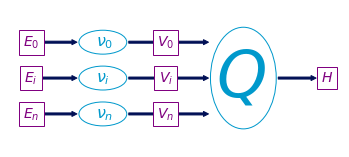
\includegraphics[width=\columnwidth]{path_of_q}
  \caption{$\vchannel_i$ functions convert data $\dsection_i$ to visual characteristics $\vsection_i$, then \vmark\ assembles $\vsection_i$ into a graphic $\gsection$ such that there is a map \vindex\ preserving the continuity of the data.} 
  \label{fig:math:artist:q}
\end{figure}
As shown in \autoref{fig:math:artist:q}, \vchannel\ and \vmark\ are a map-reduce operation: map the data into their visual encodings \vsection\ reduce the encodings into a graphic \gsection. While it may seem intuitive that visualizations that generate the same graphic should do so consistently given the same input, we formalize this constraint such that it can be specified as a constraint of \vmark. We define the equivariant map as  $\vmark: \vsection \mapsto \gsection$ and an action on the subset of graphics $\vmark(\Gamma(\vtotal)) \in \Gamma(\gtotal)$ that \vmark\ can generate. We then define the constraint on \vmark such that if \vmark\ is applied to two visual sections $\vsection,\vsection^{\prime}$ that generate the same \gsection\, then the output of $\vsection,\vsection^{\prime}$ acted on by the same monoid $m$ must be the same.

\begin{figure}[htb]
  \centering
  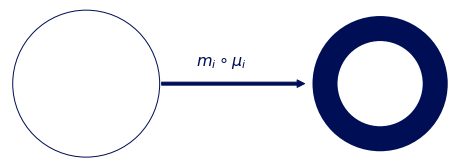
\includegraphics[width=\columnwidth]{diff_type_q.png}
  \caption{These two glyphs are generated by the same \vmark\ function. The monoid 
  action $m_i$ on edge thickness $\vsection_i$ of the first glyph yields the thicker edge ${\vsection_i}^{\prime}$ in the second glyph.}
  \label{fig:math:artist:graphic}
\end{figure}

Lets call the visual representations of the components $\Gamma(\vtotal)=X$ and the graphic $\vmark(\Gamma(\vtotal))=Y$. If for elements of the monoid $m \in \monoid$ and for all $\vsection, \vsection^{\prime} \in X$, we define the monoid action on $X$ so that it is by definition equivariant
\begin{equation}
\vmark(\vsection) = \vmark(\vsection^{\prime})\implies \vmark(m\circ\vsection) = \vmark(m\circ\vsection^{\prime})
\end{equation}
then a monoid action on $Y$ can be defined as $m\circ \gsection = \gsection^{\prime}$. The transformed graphic $\gsection^{\prime}$ is equivariant to a transform on the visual bundle $\gsection^{\prime}=\vmark(m\circ \vsection)$ on a section that $\vsection \in \vmark^{-1}(\gsection)$ that must be part of generating \gsection. Given fiber $\vfiber=(xpos,\, ypos,\, color,\, thickness)$, then sections $\vsection=(0,0,0,1)$ and $\vmark(\vsection) = \gsection$ generates a piece of the thin hollow circle. The action $m=(e, e, e, x+2)$, where e is identity, translates \vsection\ to  $\vsection^{\prime}=(e,e,e,3)$ and the corresponding action on \gsection\ causes $\vmark(\vsection^{\prime})$ to be the thicker circle in \autoref{fig:math:artist:graphic}.

We formally describe a glyph as \vmark\ applied to the regions \dbasepoint\ that map back to a set of path connected components $\dbasepath \subset \dbase$ as input 
\begin{equation}
\dbasepath = \{\dbasepathpoint \in \dbase \text{ s. t. } \exists \gamma \text{ s.t. } \gamma(0)=\dbasepoint \text{ and }\gamma(1)=\dbasepathpoint\}
\end{equation}
where the path\cite{ConnectedSpace2020}  $\gamma$ from \dbasepoint\ to \dbasepathpoint\ is a continuous function from the interval [0,1]. We define the glyph as the graphic generated by $\vmark(\gbase_{\dbasepathpoint})$
\begin{equation}
  \begin{tikzcd}
      \gtotal \arrow[r, shift left] & \gbase_\dbasepathpoint \arrow[rr, "\vindex(\gbasepoint)", shift left] \arrow[l, "\gsection(\gbase_\dbasepathpoint)"] &  & \dbasepath_{\dbasepoint} \arrow[ll, "\vindex^{-1}(\dbasepath)"]
      \end{tikzcd}
  \label{eq:mark}
\end{equation}
such that for every glyph there is at least one corresponding region on \dbase, in keeping with the definition of glyph as any differentiable element put forth by Ziemkiewicz and Kosara\cite{ziemkiewiczEmbeddingInformationVisualization2009}. The primitive point, line, and area marks\cite{bertinSemiologyGraphicsDiagrams2011a,carpendaleVisualRepresentationSemiology} are specially cased glyphs.

\begin{figure}
  \centering
  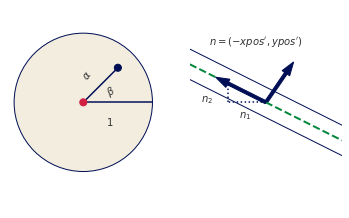
\includegraphics[width=\columnwidth]{base_q}
  \caption{The coordinates $(\gx, \gy)$ dictate the color of the region in prerender space \gbase\, which over the whole disk generates the graphical mark. The line fiber is thickened with the derivative because the tangent the line needs to be pushed perpendicular to the tangent of (xpos, ypos) in order to have visible thickness.}
  \label{fig:math:artist:base}
\end{figure}

In \autoref{fig:teaser}, we illustrate the output of a minimal Q that will generate distinguishable graphical marks: non-overlapping scatter points, a non-infinitely thin line, and an image. The scatter plot can be defined as $\vmark(xpos, ypos)(\alpha, \beta)$ where color $\gsection_{RGB} = (0,0,0)$ is defined as part of \vmark\ and $\gbasepoint=(\alpha, \beta)$ defines the region on \gbase. The position of this swatch of color can be computed relative to the location on the disc $\gbase_{\dbasepoint}$ as shown in \autoref{fig:math:artist:base}
\begin{align*}
x &= size *\alpha \cos(\beta) + xpos \\
y &= size *\alpha \sin(\beta) + ypos
\end{align*}
such that $\gsection(\gbasepoint) = (x, y, 0, 0, 0)$ colors the point (x,y) black. In contrast, the line plot $\vmark(xpos, \hat{n_{1}}, ypos, \hat{n_{2}})(\alpha, \beta)$ in \autoref{fig:teaser} has a \vindex\ function that is not only parameterized on \dbasepoint\ but also on the $\alpha$ distance along \dbasepoint\ and corresponding region in \gbase. As shown in \ref{fig:math:arist:base} line needs to know the tangent of the data to draw an envelope above and below each (xpos,ypos) such that the line appears to have a thickness. The magnitude of the slope is $\lvert n \rvert = \sqrt{{n_{1}}^2 + {n_{2}}^2}$
such that the normal is  $\hat{n_{1}} = \frac{n_1}{\lvert n \rvert}, \; \hat{n_{2}} = \frac{n_2}{\lvert n \rvert}$ which yields components of \gsection\
\begin{align*}
 x = xpos(\vindex(\alpha)) &+ width*\beta\hat{n_1}(\vindex(\alpha)) \\
 y = ypos(\vindex(\alpha)) &+ width*\beta\hat{n_2}(\vindex(\alpha)) 
\end{align*}
where (x,y) look up the position $\vindex(\alpha)$ on the data and the derivatives $\hat{n_1}, \hat{n_2}$ . The derivatives are then multiplied by a $width$ parameter to specify the thickness.

The image $\vmark(xpos, ypos, color)$ in \autoref{fig:teaser} is a direct lookup into  $\vindex:\gbase\rightarrow\dbase$. The indexing variables $(\alpha, \beta)$ define the distance along the space, which is then used by \vindex\ to map into \dbase\ to lookup the color values 
\begin{equation*}
R = R(\vindex(\alpha, \beta)), \; G = G(\vindex(\alpha, \beta)), \; B = B(\vindex(\alpha, \beta))
\end{equation*}
In the case of an image, the indexing mapper \vindex\ may do some translating to a convention expected by \vmark, for example reorientng the array such that the first row in the data is at the bottom of the graphic. 

\subsubsection{Assembly Factory}
The graphic base space \gbase\ is not accessible in many architectures, including Matplotlib; instead we can construct a factory function \vmarkd\ over \dbase\ that can build a \vmark. As shown in eq~\ref{eq:math:artist:diagram}, \vmark\ is a bundle map $\vmark: \vtotalpull\rightarrow \gtotal$ where \vtotalpull\ and \gtotal\ are both bundles over \gbase.
\begin{figure}[htb]
  \centering
    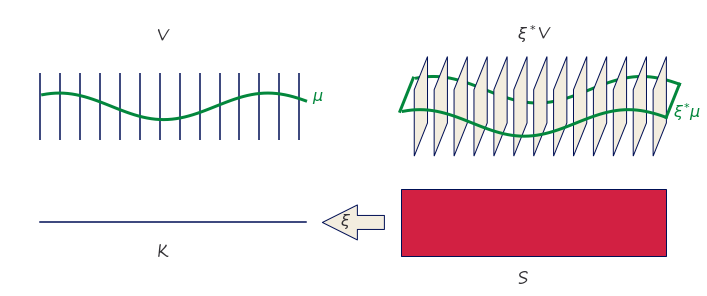
\includegraphics[width=1\columnwidth]{q_hat.png}
    \caption{Because the pullback of the visual bundle \vtotalpull\ is the replication of a \vsection\ over all points \gbasepoint\ that map back to a single \dbasepoint, we can constract a \vmarkd\ on \vsection\ over \dbasepoint\ that will fabricate the \vmark\ for the equivalent region of \gbasepoint\ associated to that \dbasepoint}
    \label{fig:math:artist:qhat}
\end{figure}

The preimage of the continuity map $\vpreimg \subset \gbase$ is such that many graphic continuity points $\gbasepoint \in \gbase_{\dbase}$ go to one data continuity point \dbasepoint; therefore, by definition the pull back of \vsection\
\begin{equation}
    \vtotalpull \mid_{\vpreimg} = \vpreimg \times \vfiber
\end{equation}
copies the visual fiber \vfiber\ over the the points \gbasepoint\ in graphic space \gbase\ that correspond to one \dbasepoint\ in data space \dbase. This set of points \gbasepoint\ are the preimage \vpreimg\ of \dbasepoint. 

As shown in \autoref{fig:math:artist:qhat}, given the section \vsectionpull\ pulled back from \vsection\ and the point $\gbasepoint \in \vpreimg$, there is a direct map $(\dbasepoint, \vsection(\dbasepoint)) \mapsto (\gbasepoint, \vsectionpull(\gbasepoint))$  from \vsection\ over \dbasepoint\ to the section \vsectionpull\ over \gbasepoint. This means that the pulled back section $\vsectionpull(\gbasepoint) = \vindex^*(\vsection(\dbasepoint))$ is the section \vsection\ copied over all \gbasepoint such that \vsectionpull\ is identical for all \gbasepoint\ where $\vindex(\gbasepoint) = \dbasepoint$. In \autoref{fig:math:artist:qhat} each dot on \vfiber\ is equivalent to the line on \vfiberpull. 

Given the equivalence between \vsection\ and \vsectionpull\ defined above, the reliance on \gbase\ can be factored out. When \vmark\ maps visual sections into graphics $\vmark: \Gamma(\vtotalpull) \rightarrow \Gamma(\gtotal)$, if we restrict \vmark\ input to \vsectionpull\ then the graphic section \gsection\ evaluated on a visual region \gbasepoint\
\begin{equation}
    \gsection(\gbasepoint) \coloneqq \vmark(\vsectionpull)(s)
    \label{eq:math:artist:qhat}
\end{equation}
 is defined as the assembly function \vmark\ with input \vsectionpull\ evaluated on \gbasepoint. Since the pulled back section \vsectionpull\ is the section \vsection\ copied over every graphic region $\gbasepoint \in \vpreimg$, we can define a \vmark\ factory function 
\begin{equation}
\label{eq:math:artist:qhat_q_s}
\vmarkd(\vsection(\dbasepoint))(\gbasepoint) \coloneqq \vmark((\vsectionpull)(\gbasepoint))
\end{equation} 
where \vmarkd\ with input \vsection\ is defined to \vmark\ that takes as input the copied section \vsectionpull\ such that both functions are evaluated over the same location $\vpreimg = \gbasepoint$ in the base space \gbase. 

Factoring out \gbasepoint\ from equation~\ref{eq:math:artist:qhat_q_s} yields $\vmarkd(\vsection(k)) = \vmark(\vsectionpull)$ where \vmark\ is no longer bound to input but \vmarkd\ is still defined in terms of \dbase. In fact, \vmarkd\ is a map from visual space to graphic space $\vmarkd:\Gamma(\vtotal) \rightarrow \Gamma(\gtotal)$ locally over \dbasepoint\ such that it can be evaluated on a single visual record  $\vmarkd:\Gamma(\vtotal_{\dbasepoint}) \rightarrow \Gamma(\gtotal\mid_{\vpreimg})$. This allows us to construct a \vmarkd\ that only depends on \dbase, such that for each $\vsection(\dbasepoint)$ there is part of $\gsection\mid_{\vpreimg}$. The construction of \vmarkd\ allows us to retain the functional map reduce benefits of \vmark\ without having to majorly restructure the existing pipeline for libraries that delegate the construction of \gsection\ to a back end such as Matplotlib.

\subsubsection{Composite and Reusable Artists}
Given the family of artists $(\dtotal_i: i\in I)$ on the same image, the + operator 
\begin{equation}
+ \coloneqq \underset{i\in I}{\sqcup} \dtotal_{i}
\end{equation}
defines a simple composition of artists. When artists share a base space $\dbase_2 \hookrightarrow \dbase_1$, a composition operator can be defined such that the artists are acting on different components of the same section. This type of composition is important for visualizations where elements update together in a consistent way, such as multiple views \cite{alboRadarComparativeEvaluation2016a, hullmanKeeping2018} and brush-linked views\cite{beckerBrushingScatterplots1987,bujaInteractiveData1991}. It is impractical to implement an artist for every single graphic; instead we implement an approximation of the equivalence class of artists $\{\vartist \in \vartist^{\prime}: \vartist_{1} \equiv \vartist_{2}\}$. Roughly, two artists are equivalent if they have the same visual fiber \vfiber\, assembly function \vmark\, and continuity map \vindex. 

\section{Prototype}
To build a prototype, we make use of the Matplotlib figure and axes artists \cite{hunterArchitectureOpenSource,hunterMatplotlib2DGraphics2007} so that we can initially focus on the data to graphic transformations and exploit the Matplotlib transform stack to transform data coordinates into screen coordinates.
\begin{minted}{python}
  fig, ax = plt.subplots()
  artist = Artist(data, transforms)
  ax.add_artist(artist)
\end{minted}
Building on the current Matplotlib artists which construct an internal representation of the graphic, \mintinline{python}{ArtistClass} acts as an equivalance class artist \vartisteq. The visual bundle \vtotal\ is specified as the \mintinline{python}{transform}dictionary of the form \mintinline{python}|{parameter:(variable, encoder)}| where parameter is a component in \vfiber, variable is a component in \dfiber,  and the \vchannel\ encoders are passed in as functions or callable objects. The data bundle \dtotal\ is passed in as a \mintinline{python}{data} object. By binding data and transforms to \vartisteq\ inside \mintinline{python}{__init__}, the \mintinline{python}{draw} method is a fully specified artist \vartist.
\begin{minted}{python}
  class ArtistClass(matplotlib.artist.Artist):
      def __init__(self, data, transforms, *args, **kwargs):
          # properties that are specific to the graphic
          self.data = data 
          self.transforms = transforms
          super().__init__(*args, **kwargs)
  
      def assemble(self, **args):
          # set the properties of the graphic
  
      def draw(self, renderer):
          # returns K, indexed on fiber then key 
          view = self.data.view(self.axes) 
          # visual channel encoding applied fiberwise 
          visual = {p: t['encoder'](view[t['name']])
                    for p, t in self.transforms.items()}
          self.assemble(**visual)
          # pass configurations off to the renderer
          super().draw(renderer)
  \end{minted}
 The data is fetched in section \dsection\ via a \mintinline{python}{view} method on the data because the input to the artist is a section on \dtotal. The \mintinline{python}{view} method takes the \mintinline{python}{axes} attribute because it provides the region in graphic coordinates \gbase\ that can be used to query back into data to select a subset. To ensure the integrity of the section, \mintinline{python}{view} must be atomic, which means that the values cannot change after the method is called in draw until a new call in draw. We put this constraint on the return of the \mintinline{python}{view} method so that we do not risk race conditions. 
 
 The \vchannel\ functions are then applied to the data to generate the visual section \vsection\ that here is the object \mintinline{python}{visual}. The conversion from data to visual space is simplified here to directly show that it is the encoding \vchannel\ applied to the component. The \mintinline{python}{assemble} function that is \vmarkd is responsible for generating a representation such that it could be serialized to recreate a static version of the graphic. This artist is not optimized because we prioritized demonstrating the separability of \vchannel\ and \vmarkd. The last step in the artist function is handing itself off to the renderer. The extra \mintinline{python}{*arg, **kwargs} arguments in \mintinline{python}{__init__,draw} are artifacts of how these objects are currently implemented.

 \subsection{Scatter and Line Artists}
 \begin{figure}[H]
    \centering 
    \subfloat[\label{fig:code:scatter}]{%
      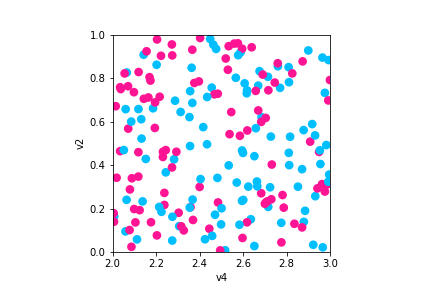
\includegraphics[width=0.49\columnwidth]{scatter_0.png}}
    \subfloat[\label{fig:code:line}]{%
      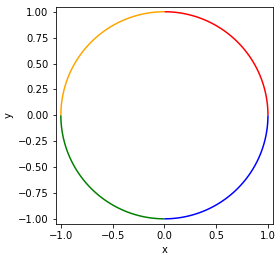
\includegraphics[width=0.49\columnwidth]{line_1.png}}
  \caption{Scatter plot and line plot implemented using prototype artists and data models, building on Matplotlib rendering.}
  \label{fig:code_scatter_line}
\end{figure}

To generate the figure in \autoref{fig:code:scatter}, the \mintinline{python}{Point} artist builds on \mintinline{python}{collection} artists because collections are optimized to efficiently draw a sequence of primitive point and area marks. In this prototype, the scatter marker shape is fixed as a circle, and the only visual fiber components are x and y position, size, and the facecolor of the marker. We only show the \mintinline{python}{assemble} function here because the \mintinline{python}{__init__, draw} are identical the prototype artist. The \mintinline{python}{view} method repackages the data as a fiber component indexed table of vertices. Even though the \mintinline{python}{view} is fiber indexed, each vertex at an index \dbasepoint has corresponding values in section $\dsection(\dbasepoint_{i})$. This means that all the data on one vertex maps to one glyph.
\begin{minted}{python}
class Point(mcollections.Collection):
  def assemble(self, x, y, s, facecolors='C0' ):
    # construct geometries of circle glyphs
    self._paths = [mpath.Path.circle((xi,yi), radius=si) 
                for (xi, yi, si) in zip(x, y, s)] 
    # set attributes of glyphs, these are vectorized 
    # circles and facecolors are lists of the same size
    self.set_facecolors(facecolors)
\end{minted} 
In \mintinline{python}{assemble}, the \vsection\ components are used to construct the vector path of each circular marker with center \texttt{(x,y)} and size \texttt{x} and set the colors of each circle. This is done via the \mintinline{python}{Path.circle} object. 
\begin{minted}{python}
class Line(mcollections.LineCollection):
    def assemble(self, x, y, color='C0'):
            #assemble line marks as set of segments 
            segments = [np.vstack((vx, vy)).T for vx, vy 
                        in zip(x, y)]
            self.set_segments(segments)
            self.set_color(color)
\end{minted}
To generate \autoref{fig:code:line}, the \mintinline{python}{Line} artist \mintinline{python}{view} method returns a table of edges. Each edge consists of (x,y) points sampled along the line defined by the edge and information such as the color of the edge. As with \mintinline{python}{Point}, the data is then converted into visual variables. In \mintinline{python}{assemble}, this visual representation is composed into a set of line segments, where each segment is the array generated by \mintinline{python}{np.vstack((vx, vy))}. Then the colors of each line segment are set. The colors are guaranteed to correspond to the correct segment because of the atomicity constraint on view. 

\subsubsection{Visual Encoders}
The visual parameter serves as the dictionary key because the visual representation is constructed from the encoding applied to the data  $\vsection = \vchannel \circ \dsection$. For the scatter plot, the mappings for the visual fiber components $\vfiber=(x,y, facecolors, s)$ are defined as
\begin{minted}{python}
cmap =  color.Categorical({'true':'deeppink', 
                           'false':'deepskyblue'})
transforms = {'x': {'name': 'v4', 'encoder': lambda x: x},
              'y': {'name': 'v2', 'encoder': lambda x: x},
              'facecolors': {'name':'v3', 'encoder': cmap}, 
              's':{'name': None , 
                   'encoder': lambda _: itertools.repeat(.02)}}
\end{minted}

where \mintinline{python}{lambda x: x} is an identity \vchannel, \mintinline{python}|{'name':None}| maps into \vfiber\ without corresponding \dsection\ to set a constant visual value, and \mintinline{python}{color.Categorical} is a custom \vchannel\ implemented as a class for reusability.  A test for equivariance can be implemented trivially
\begin{minted}{python}
def test_nominal(values, encoder):
    m1 = list(zip(values, encoder(values)))
    random.shuffle(values)
    m2 = list(zip(values, encoder(values)))
    assert sorted(m1) == sorted(m2)
\end{minted}
but is currently factored out of the artist for clarity. 

\subsubsection{Data Model}
The data input into the \mintinline{python}{Artist} will often be a wrapper class around an existing data structure. This wrapper object must specify the fiber components \dfiber\ and connectivity \dbase\ and have a \mintinline{python}{view} method that returns an atomic object that encapsulates \dsection. To support specifying the fiber bundle, we define a \mintinline{python}{FiberBundle} data class\cite{DataclassesDataClasses}

\begin{minted}{python}
@dataclass
class FiberBundle:
    K: dict #{'tables': []}
    F: dict #  {variable name: type}
\end{minted}
that asks the user to specify the the properties of \dfiber\ and the \dbase\ connectivity in terms of a  simplicial triangulation scheme \cite{geometricaSimplicialComplexes}. To generate the scatter plot and the line plot, the distinction is in the \mintinline{python}{tau} method that is the section. 
\begin{minted}{python}
class VertexSimplex: 
    """Fiberbundle is consistent across all sections
    """
    FB = FiberBundle({'tables': ['vertex']},  
            {'v1': float, 'v2': str, 'v3': float})
            
    def __init__(self, sid = 45, size=1000, max_key=10**10):
        # create random list of keys
    def tau(self, k):
      # e1 is sampled from F1, e2 from F2, etc...
      return (k, (e1, e2, e3, e4))
\end{minted}
The discrete \mintinline{python}{tau} method returns a record of discrete points, while the line\mintinline{python}{tau} returns a sampling of points along an edge \dbasepoint
\begin{minted}{python}
def tau(self, k): #will fix location on page on revision
    x, y = self._xy(k, self.distances, 
               self.angle_samples[k], self.angle_samples[k+1]) 
    color = self._color(k) 
    return (k, (x, y, color))
\end{minted}
In both cases the \mintinline{python}{view} method packages the data
\begin{minted}{python}
  def view(self, axes):
      table = defaultdict(list)
      for k in self.keys:
          table['index'].append(k)
          for (name, value) in zip(self.FB.fiber.keys(), 
                                   self.tau(k)[1]):
              table[name].append(value)
      return table
\end{minted}
into a data structure that the artist can unpack via data component name. 

\begin{figure}[htb]
  \centering 
  \subfloat[\label{fig:code:line:arc}]{%
    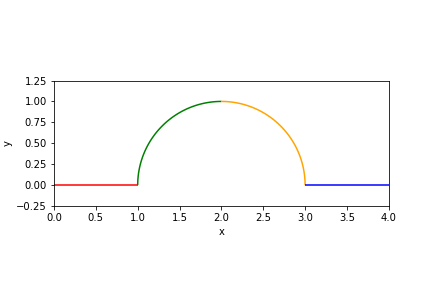
\includegraphics[width=0.49\columnwidth]{linec_1.png}}
  \subfloat[\label{fig:code:line:step}]{%
    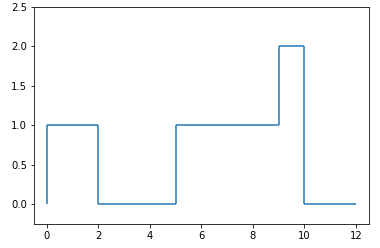
\includegraphics[width=0.49\columnwidth]{lined_1.png}}
\caption{Continuous and discontinuous lines as defined via the same data model, and generated with the same \vartisteq \mintinline{python}{Line}}
\label{fig:code:multilines}
\end{figure}
The graphics in figure~\ref{fig:code:multilines} are made using the \mintinline{python}{Line} artist and the \mintinline{python}{Graphline} data source where if told that the data is connected, the data source will check for that connectivity by constructing an adjacency matrix. The multicolored line is a connected graph of edges with each edge function evaluated on 1000 samples, 
\begin{minted}{python}
simplex.GraphLine(FB, edges, verticies, 
                      num_samples=1000, connect=True)
\end{minted}
while the stair chart is discontinuous and only needs to be evaluated at the edges of the interval 
\begin{minted}{python}
simplex.GraphLine(FB, edges, verticies, 
                      num_samples=2, connect=False)
\end{minted}
such that one advantage of this model is it helps differentiate graphics that have different artists from graphics that have the same artist but make different assumptions about the source data. 

\section{Discussion}
This work contributes a mathematical description of the mapping \vartist\ from data to visual representation. Combining Butler's proposal of a fiber bundle model of visualization data with Spivak's formalism of schema lets this model support a variety of datasets, including  discrete relational tables,, multivariate high resolution spatio temporal datasets, and complex networks. Decomposing the artist into encoding \vchannel, assembly \vmark, and reindexing \vindex\ provides the specifications that the graphic must have continuity equivalent to the data, and that the visual characteristics of the graphics are equivariant to their corresponding components under monoid actions. This model defines these constraints on the transformation function such that they are not specific to any one type of encoding or visual characteristic. Encoding the graphic space as a fiber bundle provides a structure rich abstraction of the target graphical design in the target display space. The toy prototype built using this model validates that is usable for a general purpose visualization tool since it can be iteratively integrated into the existing architecture rather than starting from scratch. Factoring out graphic formation into assembly functions allows for much more clarity in how they differ. This prototype demonstrates that this framework can generate the fundemental point (scatter plot) and line (line chart) marks. 

\subsection{Limitations}
So far this model has only been worked out for a single data set tied to a primitive mark. The examples and prototype have so far only been implemented for the static 2D case, but nothing in the math limits to 2D and expansion to the animated case should be possible because the model is formalized in terms of the sheaf. While this model supports equivariance of figurative glyphs generated from parameters of the data\cite{beckfeathers2014,byrneFigurativeFramesCritical2017}, it does not have a way to evaluate the semantic accuracy of the figurative representation. Even though the model is designed to be backend and format independent, it has only really been tested against PNGs rendered with the AGG backend. It is especially unknown how this framework interfaces with high performance rendering libraries such as openGL\cite{CarsonOpenGL1997}. This model and the associated prototype is deeply tied to Matplotlib's existing architecture, so it has not been worked through how the model generalizes to other libraries, such as those built on Mackinlay's APT framework.

\subsection{Future Work}
More work is needed to formalize the composition operators and equivalence class \vartisteq.  More artists need to be implemented to demonstrate that the model can underpin a minimally viable library,  foremost an image\cite{toryRethinkingVisualizationHighlevel2004, haber1990visualization,hansen2011visualization}, a heatmap\cite{wilkinsonHistoryClusterHeat2009,loua1873atlas}, and an imherently computational artist such as the boxplot\cite{wickham40YearsBoxplots2011}. This could be pushed further to integrate with topological\cite{heineSurveyTopologybasedMethods2016} and functional \cite{ramsayFunctionalDataAnalysis2006a} data analysis methods. Since this model formalizes notions of structure preservation, it can serve as a good base for tools that assess quality metrics\cite{bertiniQualityMetricsHighdimensional2011a} or invariance \cite{kindlmannAlgebraicProcessVisualization2014} of visualizations with respect to graphical encoding choices. While this paper formulates visualization in terms of monoidal action homomorphisms between fiberbundles, the model lends itself to a categorical formulation\cite{fongInvitationAppliedCategory2019,milewskiCategoryTheoryProgrammers} that could be further explored. 
\section{Conclusion}
An unoffical philosophy of Matplotlib is to support making whatever kinds of plots a user may want, even if they seem nonsensical to the development team. The topological framework described in this work provides a way to facilitate this graph creation in a rigorous manner; any artist that meets the equivariance criteria described in this work by definition generates a graphic representation that matches the structure of the data being represented. We leave it to domain specialists to define the structure they need to preserve and the maps they want to make, and hopefully make the process easier by untangling these components into seperate constrained maps and providing a fairly general data and display model. 

%% if specified like this the section will be committed in review mode
\acknowledgments{
The authors wish to thank the Matplotlib development team for their invaluable feedback along the way, particulary Bruno Beltran for discussions about the visual fiber space. This project has been made possible in part by grant number 2019-207333 from the Chan Zuckerberg Initiative DAF, an advised fund of Silicon Valley Community Foundation.}

%\bibliographystyle{abbrv}
\bibliographystyle{abbrv-doi}
%\bibliographystyle{abbrv-doi-narrow}
%\bibliographystyle{abbrv-doi-hyperref}
%\bibliographystyle{abbrv-doi-hyperref-narrow}
\bibliography{../draft/glasslab_viz.bib}

\end{document}

